%!TEX root = ../main.tex

\section{The Large Hadron Collider}
\label{sec:detector:lhc}

At CERN elementary particle physics is studied using the world's largest
particle accelerator, the Large Hadron Collider (LHC). Located at the
French-Swiss border area an accelerator complex including several linear and
circular (pre-)accelerators is operated (see
\cref{fig:detector:accelerators}).
\begin{figure}
\centering
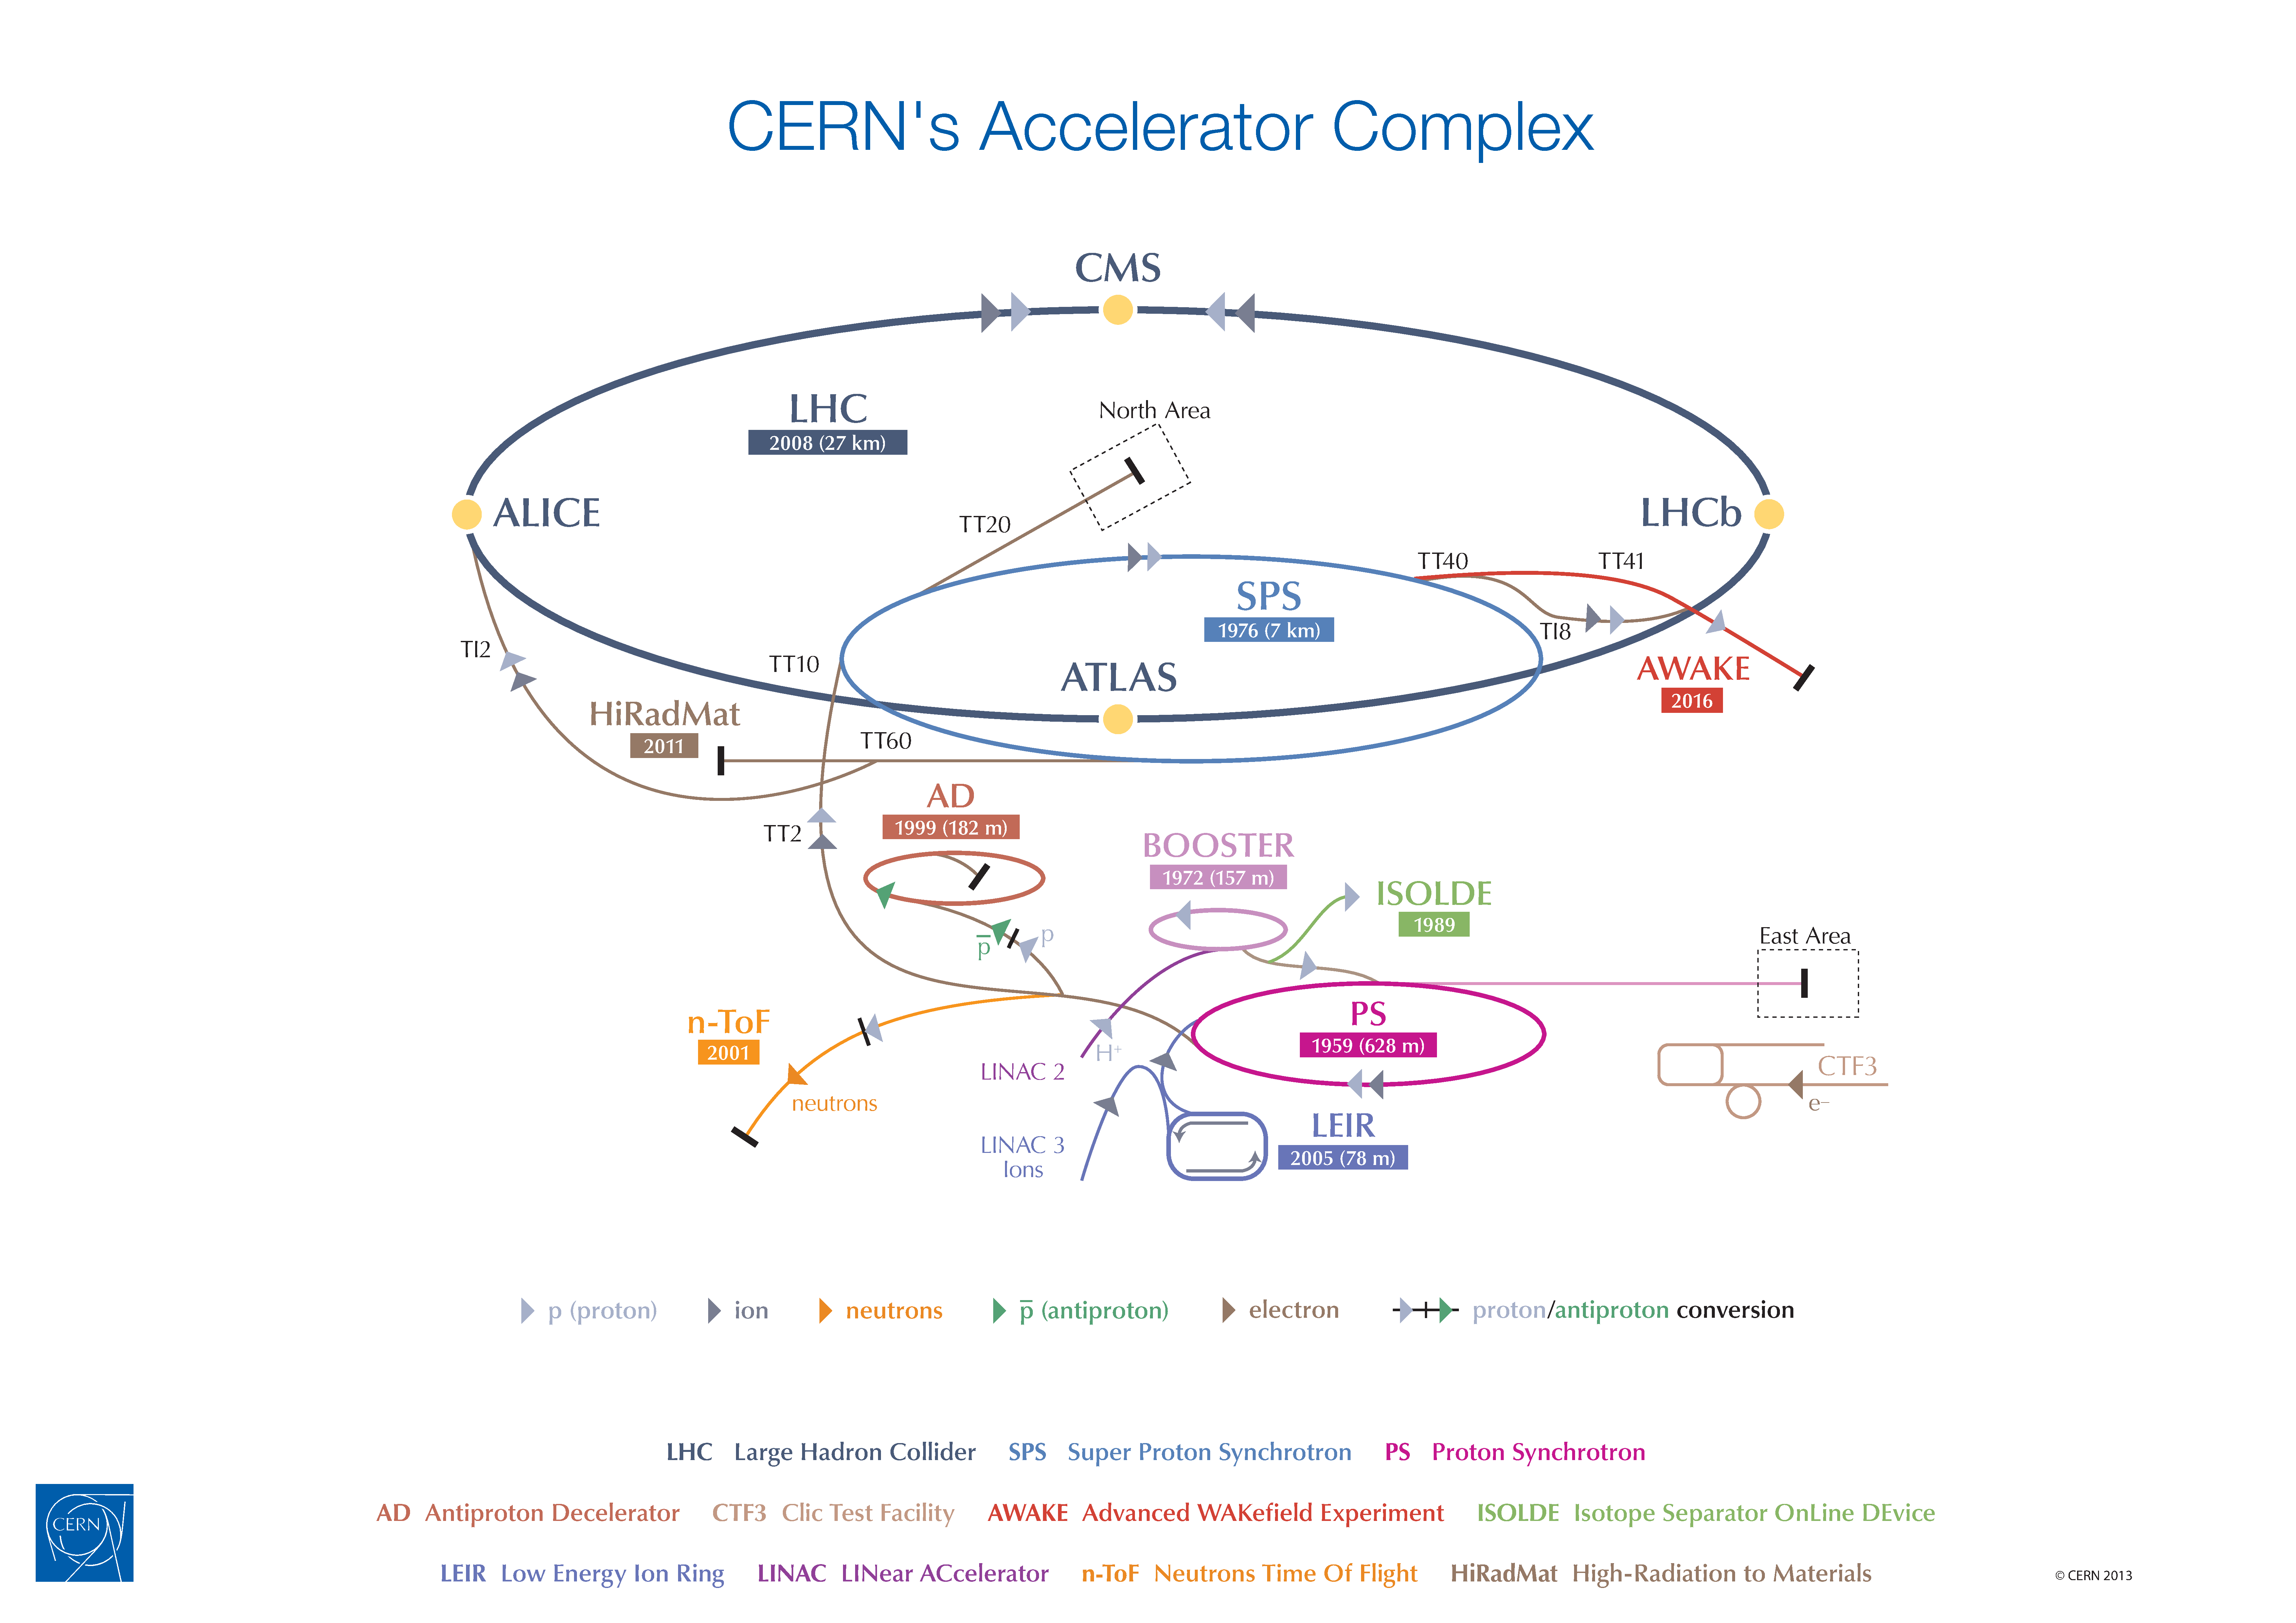
\includegraphics[width=0.8\textwidth]{04-Detector/figs/CERN_complex.pdf}
\caption{CERN's accelerator complex~\cite{Marcastel:1621583}.}
\label{fig:detector:accelerators}
\end{figure}
Before particles enter the \SI{27}{\kilo\metre} long ring of the LHC
\SIrange[range-phrase={\,to\,}]{50}{175}{m} beneath ground, they have undergone
accelerations to an energy of \SI{450}{\gev} by the linear accelerator LINAC
2, the BOOSTER, the Proton Synchrotron (PS) and the Super Proton Synchrotron
(SPS). A total of 1232 superconducting dipole magnets keep the particle beams
on the circular track, while quadrupole magnets focus them. The magnets have
to be operated at a temperature of
\SI{-271.3}{\celsius}, which is achieved by a cooling system of liquid
helium.

From 2010 on mainly proton bunches and for shorter periods of time also
bunches of lead, on whose study ALICE (A Large Ion Collider
Experiment)~\cite{ALICE} is focused, are injected. The protons are collided at
centre-of-mass energies of \SIlist{7;8}{\TeV} in 2011 and 2012 (Run I) and
since 2015 (Run II) at \SI{13}{\TeV}.